\documentclass[12pt]{article}
\usepackage{graphicx,float}
\usepackage[section]{placeins}
\usepackage{enumerate}
\usepackage{amsmath}
\usepackage{amssymb}
\pagenumbering{gobble}

\title{EE230: Lab 6\\
Non-idealities in Op-Amp}
\author{Prateek Garg, 20D070060}
\begin{document}
\maketitle

\section{Overview of the experiment}
\subsection{Aim of the experiment}
Measure the types of non-idealities like offset voltage and 
current in an op-amp(UA741) and also to find open loop gain by making circuits on breadboard .

\subsection{Methods}
The goal was to formulate and measure the offset voltage, bias currents and DC open-loop gain
 that affect the characteristics of a non-ideal op-amp. We used various circuits to neglect effect 
 of two things to approximate the third non ideality as given in labsheet.

\newpage

 \section{Design}


 \subsection{Offset Voltage and Bias Currents}

\begin{figure}[H]
    \centering
    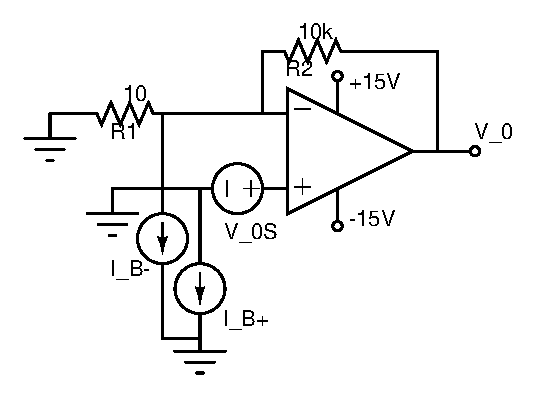
\includegraphics[scale=1]{fig2.eps}
    \caption{Circuit for measurement of $V_{OS}$}
    \label{fig:1a}
\end{figure}


\begin{figure}[H]
    \centering
    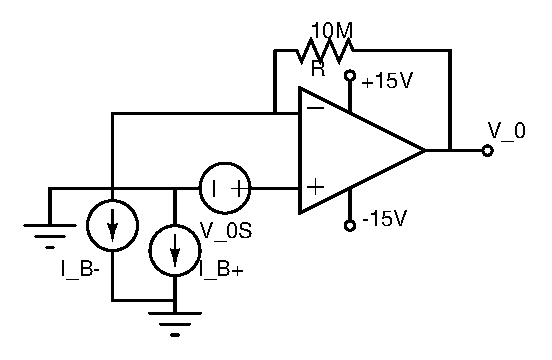
\includegraphics[scale=1]{fig4.eps}
    \caption{Circuit for measurement of $I^-_B$}
    \label{fig:1b}
\end{figure}


\begin{figure}[H]
    \centering
    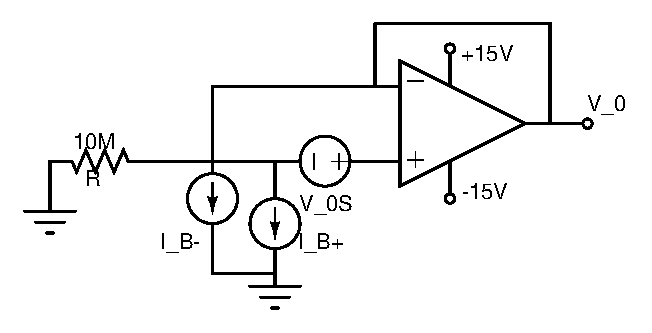
\includegraphics[scale=1]{fig6.eps}
    \caption{Circuit for measurement of $I^+_B$}
    \label{fig:1c}
\end{figure}


\subsection{DC Open Loop Gain}


\begin{figure}[H]
    \centering
    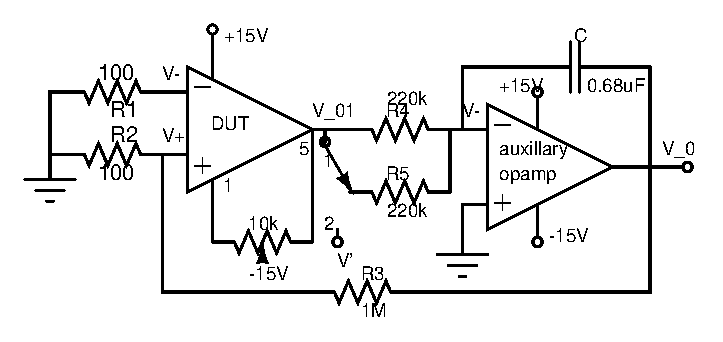
\includegraphics[scale=1]{fig8.eps}
    \caption{Circuit for measurement of $A_{OL}$}
    \label{fig:2}
\end{figure}
\section{Experimental results}
\begin{table}[!hbt]
		% Center the table
		\begin{center}
		\caption{Offset Voltage}
		\begin{tabular}{|c|c|c|c|}
			% To create a horizontal line, type \hline
			\hline
			% To end a column type &
			% For a linebreak type \\
			Characteristic & Observed \\
			\hline
			V_{o}  & $\approx$ 0.3V   \\
			\hline
			V_{OS}   & $\approx$ 0.3mV   \\
			\hline
		    
            
		\end{tabular}
		\end{center}
\end{table}



\newpage

\begin{table}[!hbt]
		% Center the table
		\begin{center}
		\caption{Ib-}
		\begin{tabular}{|c|c|c|c|}
			% To create a horizontal line, type \hline
			\hline
			% To end a column type &
			% For a linebreak type \\
			Characteristic & Observed \\
			\hline
			V_{o}  & $\approx$ 0.213V   \\
			\hline
			R   & $\approx$ 10M\Omega   \\
			\hline
			I_{B}^{-}   & $\approx$ 21.6nA   \\
			\hline
		    
            
		\end{tabular}
		\end{center}
\end{table}

\begin{table}[!hbt]
		% Center the table
		\begin{center}
		\caption{Ib+}
		\begin{tabular}{|c|c|c|c|}
			% To create a horizontal line, type \hline
			\hline
			% To end a column type &
			% For a linebreak type \\
			Characteristic & Observed \\
			\hline
			V_{o}  & $\approx$ -0.382V   \\
			\hline
			R   & $\approx$ 10M\Omega   \\
			\hline
			I_{B}^{+}   & $\approx$ -38.2nA   \\
			\hline
		    
            
		\end{tabular}
		\end{center}
\end{table}

\begin{table}[!hbt]
	\begin{center}
	\caption{Readings\\}
	\begin{tabular}{|c|c|c|}
		\hline
		$V'$ & $V_{oB}-V_{oA}$ & $A_{OL}$\\
		\hline
        $1\ V$ & $-119\ mV$ & $8.33\times10^4$\\
		\hline
        $2\ V$ & $-153\ mV$ & $12.98\times10^4$\\
		\hline
        $3\ V$ & $-198\ mV$ & $15\times10^4$\\
		\hline
	\end{tabular}
	\end{center}
\end{table}

\end{document}